\documentclass{ximera}

%\usepackage{todonotes}

\newcommand{\todo}{}


\graphicspath{
{./}
{../functionsOfSeveralVariables/}
{../normalVectors/}
{../lagrangeMultipliers/}
}


\usepackage{tkz-euclide}
\tikzset{>=stealth} %% cool arrow head
\tikzset{shorten <>/.style={ shorten >=#1, shorten <=#1 } } %% allows shorter vectors

\usetikzlibrary{backgrounds} %% for boxes around graphs
\usetikzlibrary{shapes,positioning}  %% Clouds and stars
\usetikzlibrary{matrix} %% for matrix
\usepgfplotslibrary{polar} %% for polar plots
\usetkzobj{all}
\usepackage[makeroom]{cancel} %% for strike outs
%\usepackage{mathtools} %% for pretty underbrace % Breaks Ximera
\usepackage{multicol}





\usepackage{array}
\setlength{\extrarowheight}{+.1cm}   
\newdimen\digitwidth
\settowidth\digitwidth{9}
\def\divrule#1#2{
\noalign{\moveright#1\digitwidth
\vbox{\hrule width#2\digitwidth}}}





\newcommand{\RR}{\mathbb R}
\newcommand{\R}{\mathbb R}
\newcommand{\N}{\mathbb N}
\newcommand{\Z}{\mathbb Z}

\newcommand{\sage}{\textsf{SageMath}}


%\renewcommand{\d}{\,d\!}
\renewcommand{\d}{\mathop{}\!d}
\newcommand{\dd}[2][]{\frac{\d #1}{\d #2}}
\newcommand{\pp}[2][]{\frac{\partial #1}{\partial #2}}
\renewcommand{\l}{\ell}
\newcommand{\ddx}{\frac{d}{\d x}}

\newcommand{\zeroOverZero}{\ensuremath{\boldsymbol{\tfrac{0}{0}}}}
\newcommand{\inftyOverInfty}{\ensuremath{\boldsymbol{\tfrac{\infty}{\infty}}}}
\newcommand{\zeroOverInfty}{\ensuremath{\boldsymbol{\tfrac{0}{\infty}}}}
\newcommand{\zeroTimesInfty}{\ensuremath{\small\boldsymbol{0\cdot \infty}}}
\newcommand{\inftyMinusInfty}{\ensuremath{\small\boldsymbol{\infty - \infty}}}
\newcommand{\oneToInfty}{\ensuremath{\boldsymbol{1^\infty}}}
\newcommand{\zeroToZero}{\ensuremath{\boldsymbol{0^0}}}
\newcommand{\inftyToZero}{\ensuremath{\boldsymbol{\infty^0}}}



\newcommand{\numOverZero}{\ensuremath{\boldsymbol{\tfrac{\#}{0}}}}
\newcommand{\dfn}{\textbf}
%\newcommand{\unit}{\,\mathrm}
\newcommand{\unit}{\mathop{}\!\mathrm}
\newcommand{\eval}[1]{\bigg[ #1 \bigg]}
\newcommand{\seq}[1]{\left( #1 \right)}
\renewcommand{\epsilon}{\varepsilon}
\renewcommand{\iff}{\Leftrightarrow}

\DeclareMathOperator{\arccot}{arccot}
\DeclareMathOperator{\arcsec}{arcsec}
\DeclareMathOperator{\arccsc}{arccsc}
\DeclareMathOperator{\si}{Si}
\DeclareMathOperator{\proj}{\vec{proj}}
\DeclareMathOperator{\scal}{scal}
\DeclareMathOperator{\sign}{sign}


%% \newcommand{\tightoverset}[2]{% for arrow vec
%%   \mathop{#2}\limits^{\vbox to -.5ex{\kern-0.75ex\hbox{$#1$}\vss}}}
\newcommand{\arrowvec}{\overrightarrow}
%\renewcommand{\vec}[1]{\arrowvec{\mathbf{#1}}}
\renewcommand{\vec}{\mathbf}
\newcommand{\veci}{{\boldsymbol{\hat{\imath}}}}
\newcommand{\vecj}{{\boldsymbol{\hat{\jmath}}}}
\newcommand{\veck}{{\boldsymbol{\hat{k}}}}
\newcommand{\vecl}{\boldsymbol{\l}}
\newcommand{\utan}{\mathbf{\hat{t}}}
\newcommand{\unormal}{\mathbf{\hat{n}}}
\newcommand{\ubinormal}{\mathbf{\hat{b}}}

\newcommand{\dotp}{\bullet}
\newcommand{\cross}{\boldsymbol\times}
\newcommand{\grad}{\boldsymbol\nabla}
\newcommand{\divergence}{\grad\dotp}
\newcommand{\curl}{\grad\cross}
%\DeclareMathOperator{\divergence}{divergence}
%\DeclareMathOperator{\curl}[1]{\grad\cross #1}
\newcommand{\lto}{\mathop{\longrightarrow\,}\limits}


\colorlet{textColor}{black} 
\colorlet{background}{white}
\colorlet{penColor}{blue!50!black} % Color of a curve in a plot
\colorlet{penColor2}{red!50!black}% Color of a curve in a plot
\colorlet{penColor3}{red!50!blue} % Color of a curve in a plot
\colorlet{penColor4}{green!50!black} % Color of a curve in a plot
\colorlet{penColor5}{orange!80!black} % Color of a curve in a plot
\colorlet{fill1}{penColor!20} % Color of fill in a plot
\colorlet{fill2}{penColor2!20} % Color of fill in a plot
\colorlet{fillp}{fill1} % Color of positive area
\colorlet{filln}{penColor2!20} % Color of negative area
\colorlet{fill3}{penColor3!20} % Fill
\colorlet{fill4}{penColor4!20} % Fill
\colorlet{fill5}{penColor5!20} % Fill
\colorlet{gridColor}{gray!50} % Color of grid in a plot

\newcommand{\surfaceColor}{violet}
\newcommand{\surfaceColorTwo}{redyellow}
\newcommand{\sliceColor}{greenyellow}




\pgfmathdeclarefunction{gauss}{2}{% gives gaussian
  \pgfmathparse{1/(#2*sqrt(2*pi))*exp(-((x-#1)^2)/(2*#2^2))}%
}


%%%%%%%%%%%%%
%% Vectors
%%%%%%%%%%%%%

%% Simple horiz vectors
\renewcommand{\vector}[1]{\left\langle #1\right\rangle}


%% %% Complex Horiz Vectors with angle brackets
%% \makeatletter
%% \renewcommand{\vector}[2][ , ]{\left\langle%
%%   \def\nextitem{\def\nextitem{#1}}%
%%   \@for \el:=#2\do{\nextitem\el}\right\rangle%
%% }
%% \makeatother

%% %% Vertical Vectors
%% \def\vector#1{\begin{bmatrix}\vecListA#1,,\end{bmatrix}}
%% \def\vecListA#1,{\if,#1,\else #1\cr \expandafter \vecListA \fi}

%%%%%%%%%%%%%
%% End of vectors
%%%%%%%%%%%%%

%\newcommand{\fullwidth}{}
%\newcommand{\normalwidth}{}



%% makes a snazzy t-chart for evaluating functions
%\newenvironment{tchart}{\rowcolors{2}{}{background!90!textColor}\array}{\endarray}

%%This is to help with formatting on future title pages.
\newenvironment{sectionOutcomes}{}{} 



%% Flowchart stuff
%\tikzstyle{startstop} = [rectangle, rounded corners, minimum width=3cm, minimum height=1cm,text centered, draw=black]
%\tikzstyle{question} = [rectangle, minimum width=3cm, minimum height=1cm, text centered, draw=black]
%\tikzstyle{decision} = [trapezium, trapezium left angle=70, trapezium right angle=110, minimum width=3cm, minimum height=1cm, text centered, draw=black]
%\tikzstyle{question} = [rectangle, rounded corners, minimum width=3cm, minimum height=1cm,text centered, draw=black]
%\tikzstyle{process} = [rectangle, minimum width=3cm, minimum height=1cm, text centered, draw=black]
%\tikzstyle{decision} = [trapezium, trapezium left angle=70, trapezium right angle=110, minimum width=3cm, minimum height=1cm, text centered, draw=black]


\title[Dig-In:]{Curl and line integrals}

\begin{document}
\begin{abstract}
Green's Theorem is a fundamental theorem of calculus.
\end{abstract}
\maketitle

In this section we will learn the \textit{fundamental derivative} for
vector fields, as well as a new fundamental theorem of calculus.


\section{The curl of a vector field}

Calculus has taught us that knowing the derivative of a function
$f:\R\to\R$ can tell us important information about the function.  In
a similar way we have that seen that if we wish to understand a
function of several variables $F:\R^n\to\R$, then the gradient, $\grad
F$, contains similar useful information. But what if you have a vector
field
\[
\vec{F}:\R^n\to\R^n
\]
what is the natural analogue of a derivative in this setting? We will
give the answer when the vector field is two or three dimensional. You
can take another course to learn more about derivatives of
$n$-dimensional vector fields.


\begin{definition}
  In two-dimensions, given a vector field $\vec{F}:\R^2\to \R^2$, where
  \[
  \vec{F}(x,y) = \vector{M(x,y),N(x,y)}
  \]
  the \dfn{curl} is given by
  \[
  \curl \vec F = \pp[N]{x}-\pp[M]{y}.
  \]
  In three-dimensions, given a vector field $\vec{F}:\R^3\to\R^3$, where
  \[
  \vec{F}(x,y,z) = \vector{U(x,y,z)),V(x,y,z)),W(x,y,z)}
  \]
  the \dfn{curl} is given by
  \begin{align*}
  \curl \vec F &= \det
  \begin{bmatrix}
    \veci & \vecj & \veck \\
    \pp{x} & \pp{y} & \pp{z}\\
    U & V & W
  \end{bmatrix}\\
  &= \veci\left(\pp[W]{y}-\pp[V]{z}\right)-
  \vecj\left(\pp[W]{x}-\pp[U]{z}\right)+
  \veck\left(\pp[V]{x}-\pp[U]{y}\right).
  \end{align*}
\end{definition}

\begin{question}
  In two dimensions $\curl\vec{F}$ is a
  \begin{multipleChoice}
    \choice[correct]{number.}
    \choice{vector.}
  \end{multipleChoice}
  \begin{question}
    In three dimensions $\curl\vec{F}$ is a
    \begin{multipleChoice}
      \choice{number.}
      \choice[correct]{vector.}
    \end{multipleChoice}
  \end{question}
\end{question}


\begin{question}
  Consider the vector field $\vec{F}(x,y) = \vector{-y,x}$. Compute:
  \[
  \curl\vec{F}(x,y) \begin{prompt}= \answer{2}\end{prompt}
  \]
  \begin{question}
    Consider the vector field $\vec{F}(x,y,z) = \vector{-z,x,y}$. Compute:
    \[
    \curl\vec{F}(x,y,z)   \begin{prompt}
      = \vector{\answer{1},\answer{1},\answer{1}}
    \end{prompt}
    \]
  \end{question}
\end{question}

Now for something you've seen before, but in a different form.

\begin{question}
  Let $F:\R^2\to\R$. Compute:
  \[
  \curl\grad F(x,y) \begin{prompt}= \answer{0}\end{prompt}
  \]
  \begin{question}
    Let $F:\R^3\to\R$. Compute:
    \[
    \curl\grad F(x,y,z) \begin{prompt}= \vector{\answer{0},\answer{0},\answer{0}}\end{prompt}
    \] 
  \end{question}
\end{question}

\begin{question}
  When $\curl\vec{F} = \vec{0}$, then you know:
  \begin{selectAll}
    \choice[correct]{$\vec{F}$ is a gradient field.}
    \choice[correct]{$\vec{F}$ is a conserttive field.}
    \choice[correct]{$\vec{F}:\R^3\to\R^3$.}
  \end{selectAll}
  \begin{feedback}
    You can be assured that $\vec{F}:\R^3\to\R^3$, since $\vec{0}$ is
    a vector. We only know a definition for curl in two and three
    dimensions; however, the two dimensional definition is a scalar,
    not a vector. So if $\curl\vec{F} = \vec{0}$, then $\vec{F}:\R^3\to\R^3$.
  \end{feedback}
\end{question}


\subsection{What does the curl measure?}


The curl of a vector field measures the rate that the direction of
field vectors ``twist'' as $x$ and $y$ change. Imagine the vectors in
a vector field as representing the current of a river. A positive curl
at a point tells you that a ``beach-ball'' floating at the point would
be rotating in a counterclockwise direction. A negative curl at a
point tells you that a ``beach-ball'' floating at the point would be
rotating in a clockwise direction. Zero curl means that the
``beach-ball'' would not be rotating. Below we see our ``beach-ball''
with two field vectors. If $\vec{F}(x,y) = \vector{M(x,y),N(x,y)}$
\begin{image}
  \begin{tikzpicture}
    \begin{axis}[
        hide axis,
        width=2in,
        height=2in,
	ymin=-1,ymax=1,
	xmin=-1,xmax=1,
      ]
       \addplot[penColor2,thick,->] coordinates{
                (-.6,0) (-.6,.3) 
       };
       \addplot[penColor2,thick,->] coordinates{
                (.6,0) (.6,.7) 
            };


      \addplot[penColor, ultra thick, domain=0:360,smooth] ({.5*cos(x)},{.5*sin(x)});
      \draw[penColor, ultra thick,->] (axis cs: .49,-.1) -- (axis cs: .5,.1) ;
    \end{axis}
  \end{tikzpicture}
\end{image}
we see that the right field vector is larger than the left, thus
giving the ``beach-ball'' a counterclockwise rotation. Since the
length of the vector increases as we increase $x$, we also see that
\[
\pp[N]{x} > 0.
\]
In an entirely similar way, if we have
\begin{image}
  \begin{tikzpicture}
    \begin{axis}[
        hide axis,
        width=2in,
        height=2in,
	ymin=-1,ymax=1,
	xmin=-1,xmax=1,
      ]
       \addplot[penColor2,thick,->] coordinates{
                (0,.6) (.3,.6) 
       };
       \addplot[penColor2,thick,->] coordinates{
                (0,-.6) (.7,-.6) 
            };


      \addplot[penColor, ultra thick, domain=0:360,smooth] ({.5*cos(x)},{.5*sin(x)});
      \draw[penColor, ultra thick,->] (axis cs: .49,-.1) -- (axis cs: .5,.1) ;
    \end{axis}
  \end{tikzpicture}
\end{image}
we see that the bottom field vector is larger than the top, thus
giving the ``beach-ball'' a counterclockwise rotation. Since the
length of the vector decreases as we increase $y$, we also see that
\[
-\pp[M]{y} > 0
\]
Thus the curl combines $\pp[N]{x}$ and $-\pp[M]{y}$
\[
\curl\vec{F} = \pp[N]{x} - \pp[M]{y}
\]
to obtain the infintesimal rotatation of the field. The most obvious
example of a vector field with nonzero curl is $\vec{F}(x,y) =
(-y,x)$.
\begin{image}
  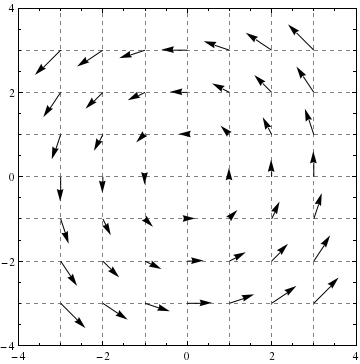
\includegraphics{rotField.png}
\end{image}
Unfortunately, while we can sometimes identify nonzero curl from a
graph, it can be difficult.

\begin{example}
  Consider the following vector field $\vec{F}$:
      \begin{image}
        \begin{tikzpicture}
          \begin{axis}%
            [
	      ymin=-2.2,ymax=2.2,
	      xmin=-3.2,xmax=3.2,
              axis lines =middle, xlabel=$x$, ylabel=$y$,
              every axis y label/.style={at=(current axis.above origin),anchor=south},
              every axis x label/.style={at=(current axis.right of origin),anchor=west},
              grid=both,
              grid style={dashed, gridColor},
              xtick={-3,...,3},
              ytick={-2,...,2},
	    ]
            \pgfplotsinvokeforeach{-2,...,2}{
              \fill[penColor] (axis cs:0,#1) circle (2pt);
              }
            \pgfplotsinvokeforeach{-2,...,1}{
              \addplot[penColor,thick,->] coordinates{
                (1,#1+.05) (1,#1+.95) 
              };
            }
            \pgfplotsinvokeforeach{-2,...,1}{
              \addplot[penColor,thick,->] coordinates{
                (-1,.95 + #1) (-1,#1+.05) 
              };
            }
            \pgfplotsinvokeforeach{-2,0}{
              \addplot[penColor,thick,->] coordinates{
                (2,#1+.05) (2,#1+1.95) 
              };
            }
            \pgfplotsinvokeforeach{-2,0}{
              \addplot[penColor,thick,->] coordinates{
                (-2,1.95 + #1) (-2,#1+.05) 
              };
            }
            \addplot[penColor,thick,->] coordinates{
                (3,-1.5) (3,1.5) 
              };
            \addplot[penColor,thick,->] coordinates{
                (-3,1.5) (-3,-1.5) 
            };

            \fill[black,draw=black] (axis cs:2,1) circle (2.5pt);

            \node[right] at (axis cs:2,1) {$\vec{a}$};
              %% \node[inner sep=0pt,text width=8cm,right,scale=.85] at (axis cs:-6,-3.5)
              %%      {\footnotesize One should imagine a vector at
              %%        \textbf{every} point. We'll assume that the magnitudes
              %%        of the vectors are constant along horizontal lines.};
          \end{axis}
        \end{tikzpicture}
      \end{image}
      Setting $\d x = 1$ and $\d y = 1$, estimate:
      \[
      \curl \vec{F}(\vec{a})
      \]
      \begin{explanation}
        First note that one should imagine a vector at \textbf{every}
        point. We'll assume that the magnitudes of the vectors are
        constant along vertical lines. Set $\vec{F}(x,y) =
        \vector{M(x,y),N(x,y)}$. To estimate $\pp[N]{x}$, we examine
        the change in $N(x,1)$ between $x=0$ and $x=1$:
        \[
        \frac{N(2,1) - N(1,1)}{2-1} = \answer[given]{1}
        \]
        and we should also check the change of $N(x,1)$ between $x=2$
        and $x=3$:
        \[
        \frac{N(3,1) - N(2,1)}{3-2} = \answer[given]{1}
        \]
        Averaging these values together we find
        \[
        \pp[N]{x} \approx \answer[given]{1}
        \]
        To estimate $\pp[M]{y}$, we examine the change in $M(2,y)$
        between $y=0$ and $y=1$:
        \[
        \frac{M(2,1) - N(2,0)}{1-0} = \answer[given]{0}
        \]
        and we should also check the change of $M(2,y)$ between $y=1$
        and $y=2$:
        \[
        \frac{M(2,2) - N(2,1)}{2-1} = \answer[given]{0}
        \]
        Averaging these values together we find
        \[
        \pp[N]{x} \approx \answer[given]{0}
        \]
        So we approximate
        \[
        \curl\vec{F}(\vec{a})\approx\answer[given]{1}.
        \]
      \end{explanation}
\end{example}

The field in the example does not have global rotation, but it does
have local rotation.

Now let's see an example where the field has global rotation, but no
local rotation.


\[
\{F:\R^2 \to \R\} \lto^{\grad} \{\vec{F}: \R^2 \to \R^2\} \lto^{\curl}
\{F:\R^2 \to \R\} 
\]



Recall,

\section{A new fundamental theorem of calculus}

\begin{theorem}[Green's Theorem]
  If $\vec{F}:\R^2\to\R^2$ has continuous partial derivatives and $C$ is a
  boundray of a closed region $R$ and $\vec{p}(t)$ paramaterizes $C$
  in a counterclockwise direction with the interior on the left, then
  \[
  \int_R \curl\vec{F}\d A = \int_C \vec{F}\dotp\d\vec{p} 
  \]
\end{theorem}

\end{document}
